\documentclass[tikz, border=10pt]{standalone}
\usepackage{pgfplots}
\usepgfplotslibrary{groupplots}
\pgfplotsset{compat=1.18}

\begin{document}
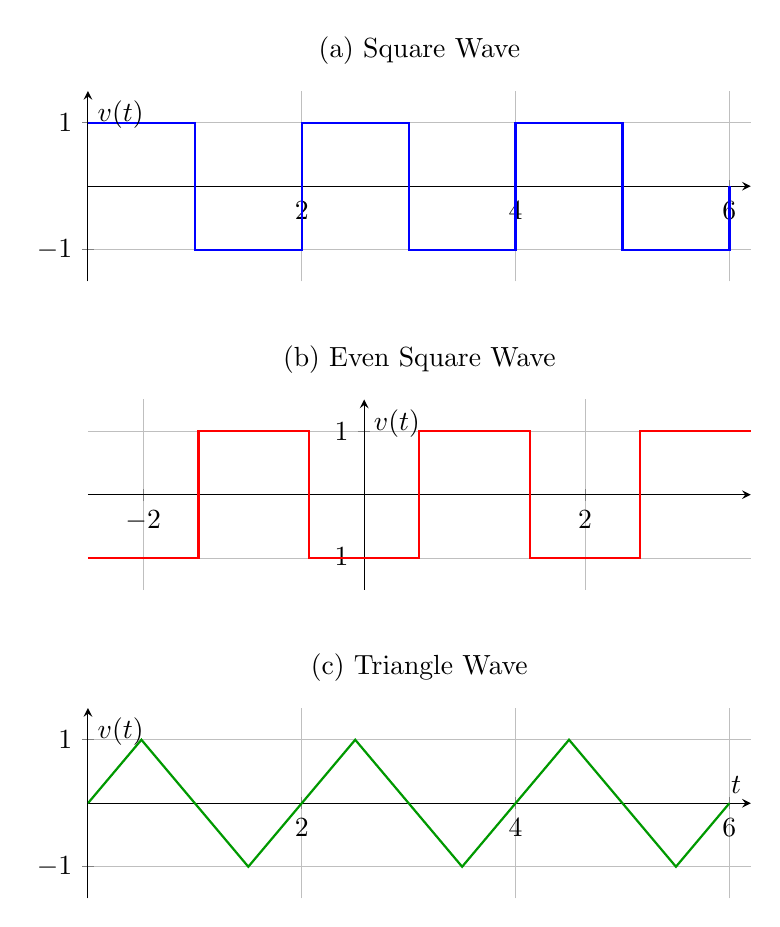
\begin{tikzpicture}
    \begin{groupplot}[
        group style={
            group size=1 by 3,
            vertical sep=1.5cm,
            xlabels at=edge bottom
        },
        width=10cm, height=4cm,
        axis lines=middle,
        xlabel={$t$}, ylabel={$v(t)$},
        ymin=-1.5, ymax=1.5,
        grid=both,
        xtick distance=0.5,
        samples=100
    ]
    
    % (a) Square wave: +1 [0,1], -1 [1,2]. Period T=2.
    \nextgroupplot[title={(a) Square Wave}, xmin=0, xmax=6.2, xtick={0,2,4,6}]
        \addplot[blue, thick] coordinates {
            (0,1) (1,1) (1,-1) (2,-1) 
            (2,1) (3,1) (3,-1) (4,-1)
            (4,1) (5,1) (5,-1) (6,-1) (6,0)
        };
        \draw[blue, dashed] (axis cs:1,1) -- (axis cs:1,-1);
        \draw[blue, dashed] (axis cs:2,-1) -- (axis cs:2,1);
        \draw[blue, dashed] (axis cs:3,1) -- (axis cs:3,-1);
        \draw[blue, dashed] (axis cs:4,-1) -- (axis cs:4,1);
        \draw[blue, dashed] (axis cs:5,1) -- (axis cs:5,-1);

    % (b) Even Square Wave: +1 [-0.5,0.5], -1 [0.5,1.5]. Period T=2.
    \nextgroupplot[title={(b) Even Square Wave}, xmin=-2.5, xmax=3.5, xtick={-2,0,2}]
        \addplot[red, thick] coordinates {
            (-2.5,-1) (-1.5,-1) (-1.5,1) (-0.5,1) (-0.5,-1) (0.5,-1) 
            (0.5,1) (1.5,1) (1.5,-1) (2.5,-1) (2.5,1) (3.5,1)
        };
        \draw[red, dashed] (axis cs:-1.5,-1) -- (axis cs:-1.5,1);
        \draw[red, dashed] (axis cs:-0.5,1) -- (axis cs:-0.5,-1);
        \draw[red, dashed] (axis cs:0.5,-1) -- (axis cs:0.5,1);
        \draw[red, dashed] (axis cs:1.5,1) -- (axis cs:1.5,-1);
        \draw[red, dashed] (axis cs:2.5,-1) -- (axis cs:2.5,1);

    % (c) Triangle Wave: 0->1 [0,0.5], 1->-1 [0.5,1.5], -1->0 [1.5,2]. Period T=2.
    \nextgroupplot[title={(c) Triangle Wave}, xmin=0, xmax=6.2, xtick={0,2,4,6}]
        \addplot[green!60!black, thick] coordinates {
            (0,0) (0.5,1) (1.5,-1) (2.5,1) (3.5,-1) (4.5,1) (5.5,-1) (6, 0)
        };

    \end{groupplot}
\end{tikzpicture}
\end{document}
